%*******10********20********30********40********50********60********70********80
\clearpage

\section{Residual Capabilities after Pure ASR Expansion}

Here the uni-axial compression test result for ASR expanded concrete model is summarised.

As an example, compression test for cases with 30\% coarse aggregate, of which 75\% are set to be ASR reactive, will be presented in details.

\begin{figure}[ht!]
\centering
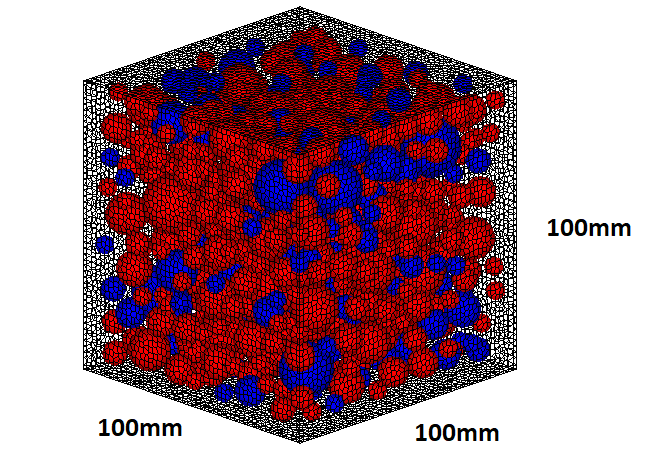
\includegraphics[width=.3\linewidth]{Files/Aggregate/A30P75.png}
  \caption{30\% Coarse Aggregate}
  \label{fig:A30P75_model}
\end{figure}

As introduced previously in chapter 2 and chapter 3, one-dimensional global expansion up to 1.3\% has been achieved by giving initial strain step by step at the interfaces between reactive aggregate and paste elements.

After expansion, three-dimensional expanded concrete models are tested under uni-axial compression condition. Displacement of loading boundary is controlled, as the top boundary of the concrete model moves downwards 0.02mm in each step. Top and bottom boundaries are under fix condition.

In each step of loading, compressive strength in the current step is recorded. As shown in Figure \ref{fig:A30P75FIX_LD}, the Load-Displacement curve obtained here is close to the shape of the normal concrete under fixed boundary compressive test, with increasing strength until reaching the maximum compressive strength, then decreasing until failure happens.

Also, in Figure \ref{fig:A30P75FIX_LD}, the trend of decreasing in maximum compressive strength along with the increasing of one-dimensional global expansion is also shown. With the global expansion increasing up to 1.3\%, the compressive strength reduced gradually to 15.993MPa, which is 53\% of undamaged model.

The Elastic Modulus, which here calculated as the maximum slope before compressive strength reaching the maximum, also shows the same trend when global expansion increase. While the Elastic Modulus is 33.8GPa for undamaged model, Elastic Modulus drop to 1.11GPa when global expansion reached 1.3\%.

Loading with free boundary condition is also simulated here, and presented in Figure \ref{fig:A30P75FREE_LD}. As the boundary are set to be without horizontal frictions, cracks are more easier to open during loading, result in a generally 30\% smaller compressive strength comparing to the result from fixed boundary loading test. This is also corrisbonding with cases in reality. A similar decreasing trend in compressive strength and elastic modulus along with the increase of global expanding ratio can be obtained.

%A30P75FIX

\begin{figure}[ht]
\centering
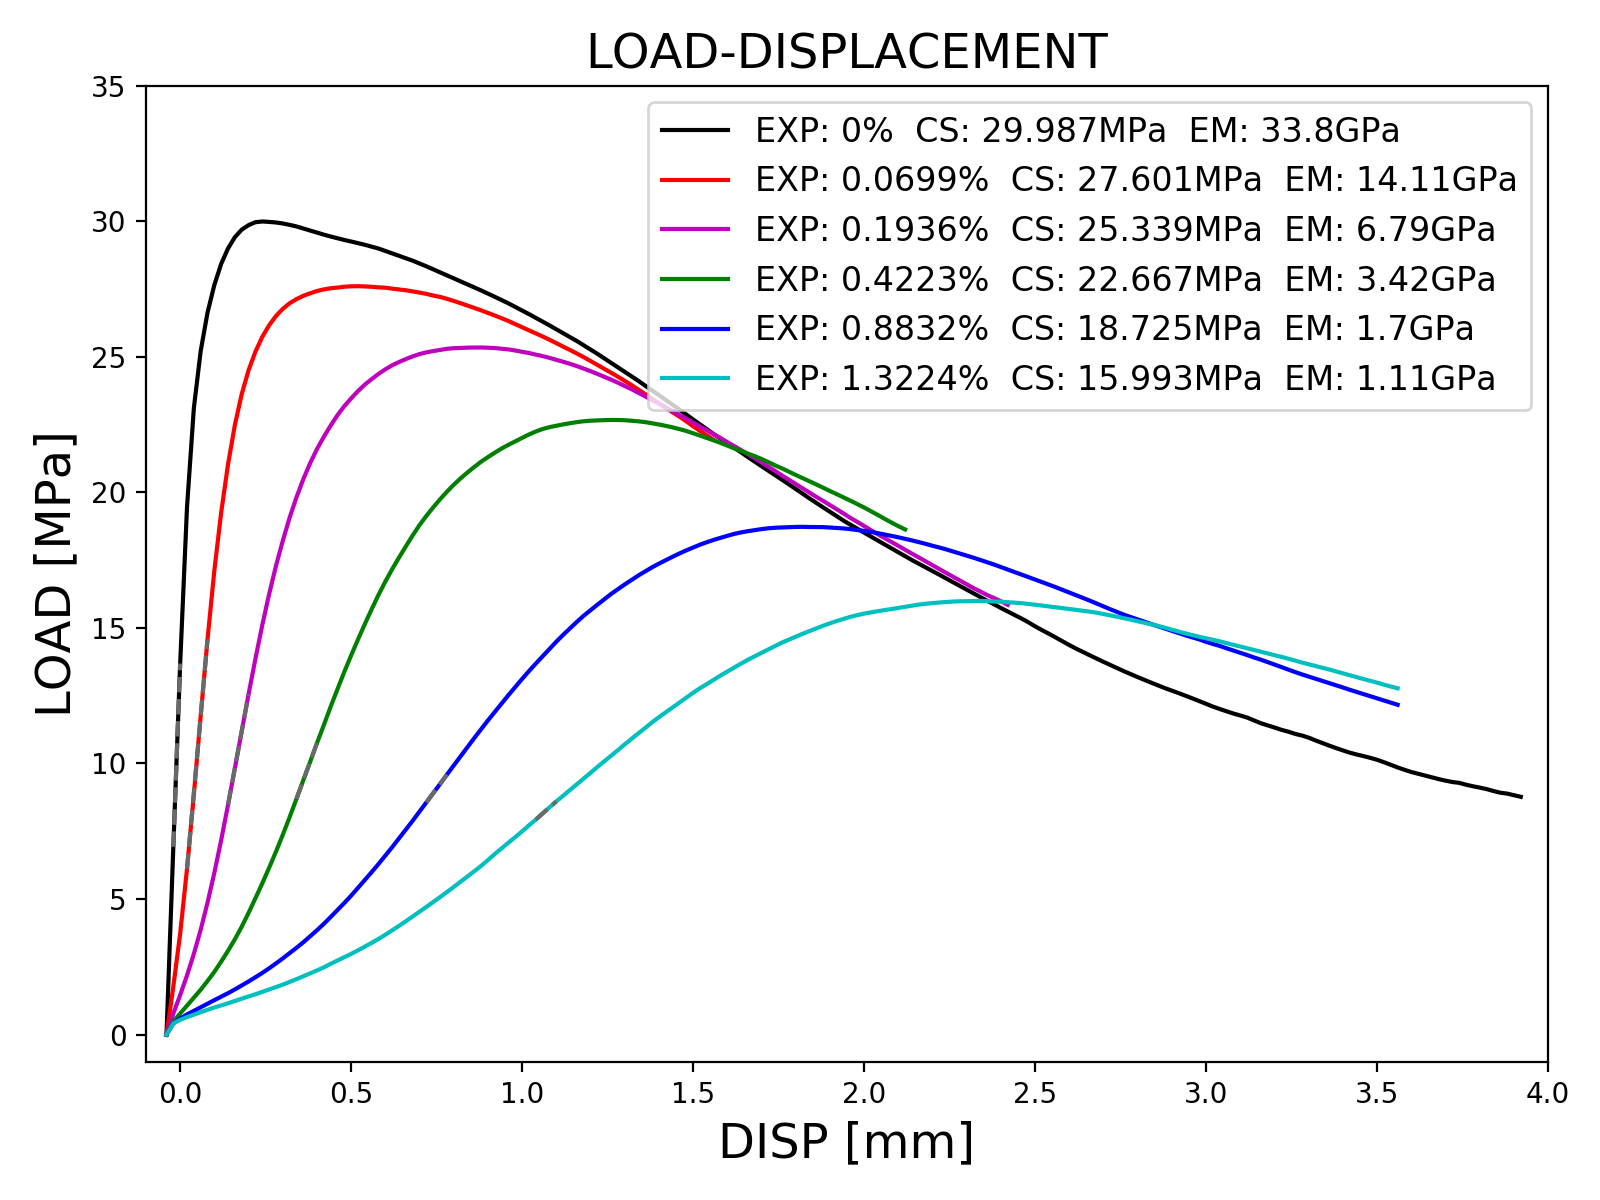
\includegraphics[width=.8\linewidth]{Files/exp_3D/ASR/S13A30P75FIX-LOAD-DISPLACEMENT.png}
  \caption{A30 P75 Fix Load-Displacement}
  \label{fig:A30P75FIX_LD}
\end{figure}

%A30P75FREE

\begin{figure}[ht!]
\centering
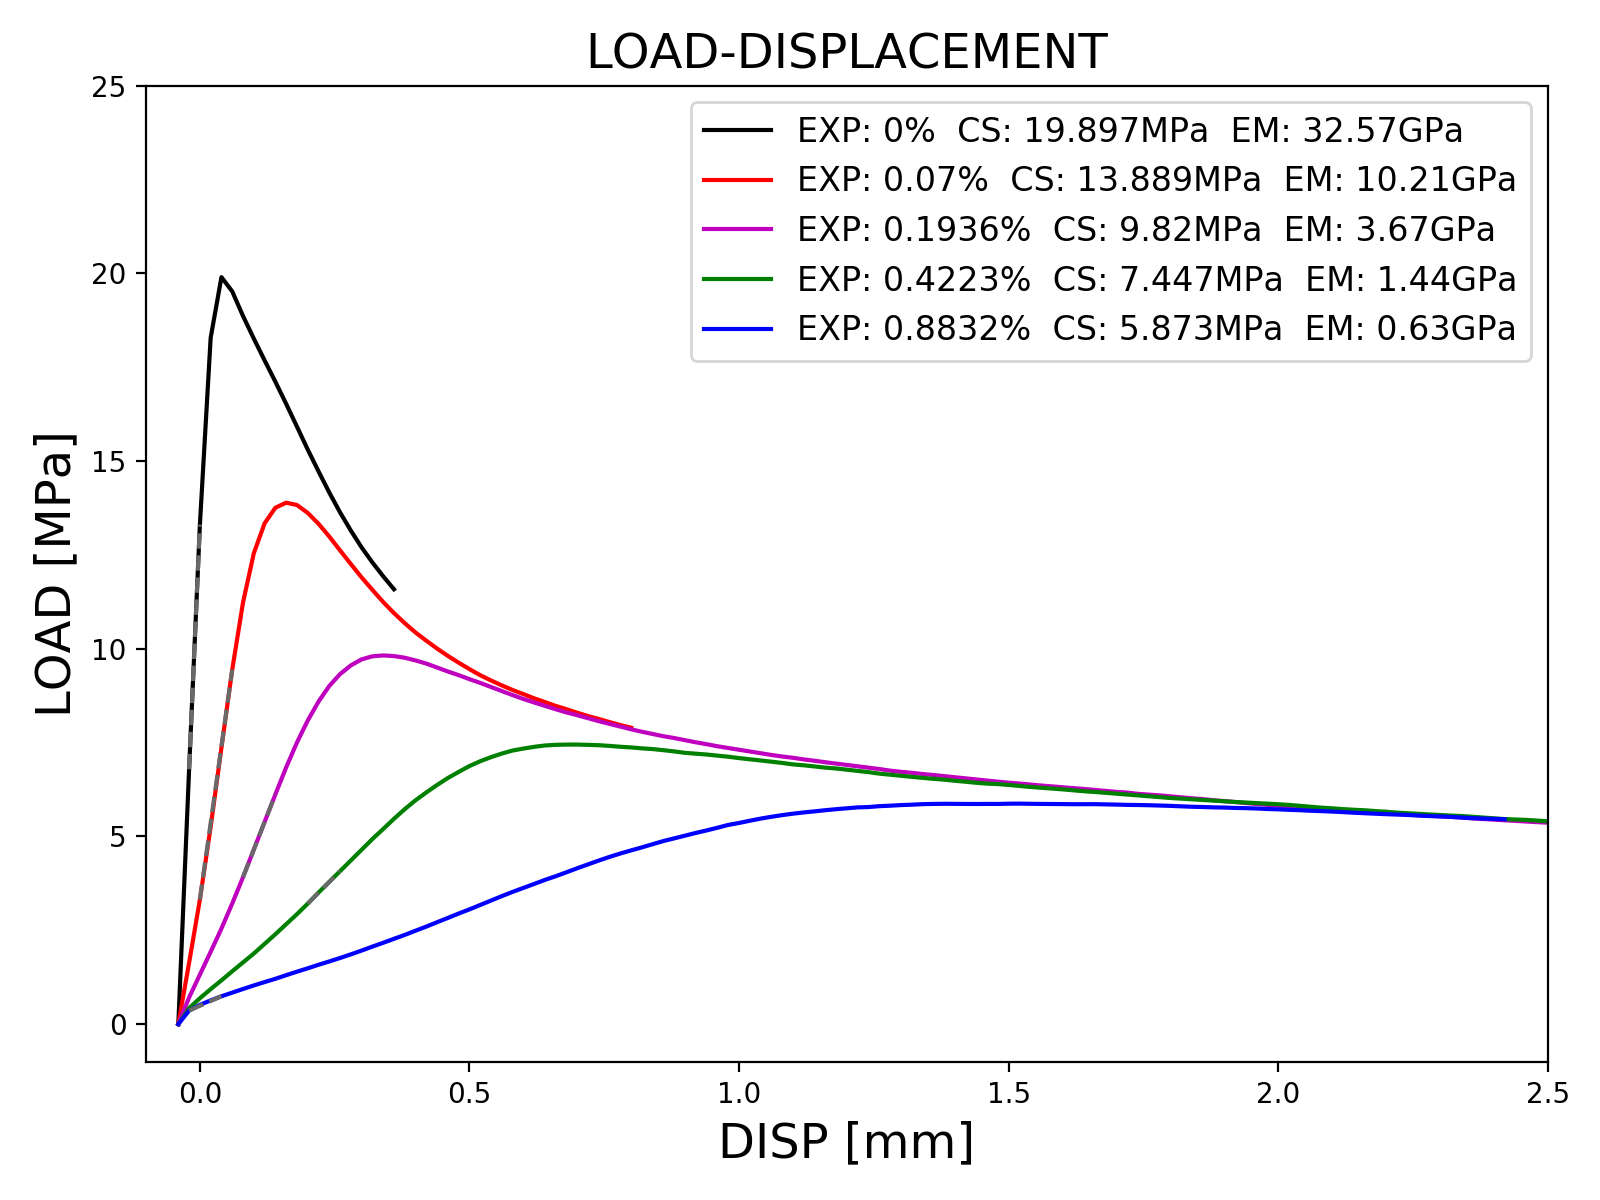
\includegraphics[width=.8\linewidth]{Files/exp_3D/ASR/S13A30P75FREE-LOAD-DISPLACEMENT.png}
  \caption{A30 P75 Free Load-Displacement}
  \label{fig:A30P75FREE_LD}
\end{figure}

% \begin{table}[ht!]
% \centering
% \begin{tabular}{ ||p{2cm}|p{2cm}|p{2cm}|p{3cm}|p{3cm}|| }
%  \hline
%   Initial Strain (Each Step) & Expanding Steps & Final Expansion [\%] & Maximum Compressive Strength in Fix Loading Condition [MPa] & Maximum Compressive Strength in Free Loading Condition [MPa]\\ [0.5ex]
%  \hline\hline
%   0 & 0 & 0 & 29.987 & 19.897\\
%   0.0002 & 20 & 0.0699 & 27.601 & 13.889\\
%   0.0005 & 20 & 0.1936 & 25.339 & 9.8203\\
%   0.001 & 20 & 0.4223 & 22.667 & 7.4466\\
%   0.002 & 20 & 0.8832 & 18.725 & 5.8732 \\
%   0.003 & 20 & 1.3224 & 15.993 &\\
%
%  \hline
% \end{tabular}
% \caption{One Dimensional Expansion Ratio in Single ASR Model Simulation}
% \label{table:ASR_30_EXP}
% \end{table}


%TODO: PLOT WITH EXPERIMENTAL RESULTS

Here the simulated compressive strength result in fixed boundary condition is compared with experimental results summarised in the beginning of this chapter.

\clearpage

Other uni-axial loading simulation results for expanded models in different cases are also summarized below.

For ASR expanded model with 30\% coarse aggregate (of which 25\% are ASR reactive), shown in Figure \ref{fig:A30P25_model}, the Load-Displacement curve is shown in Figure \ref{fig:A30P25FIX_LD}.

%A30P25FIX
\begin{figure}[ht]
\centering
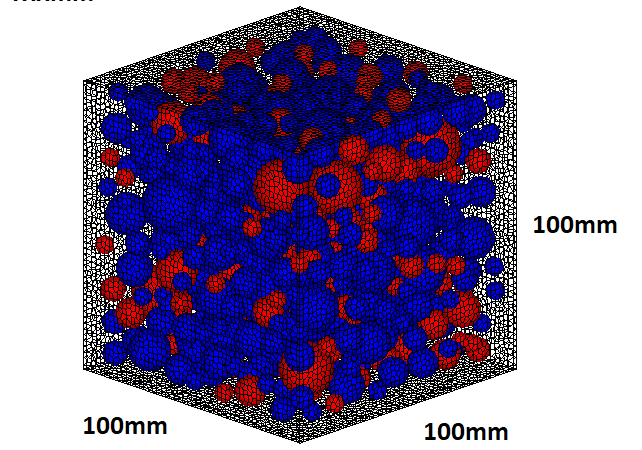
\includegraphics[width=.3\linewidth]{Files/Aggregate/A30P25.png}
  \caption{30\% Coarse Aggregate}
  \label{fig:A30P25_model}
\end{figure}

\begin{figure}[ht]
\centering
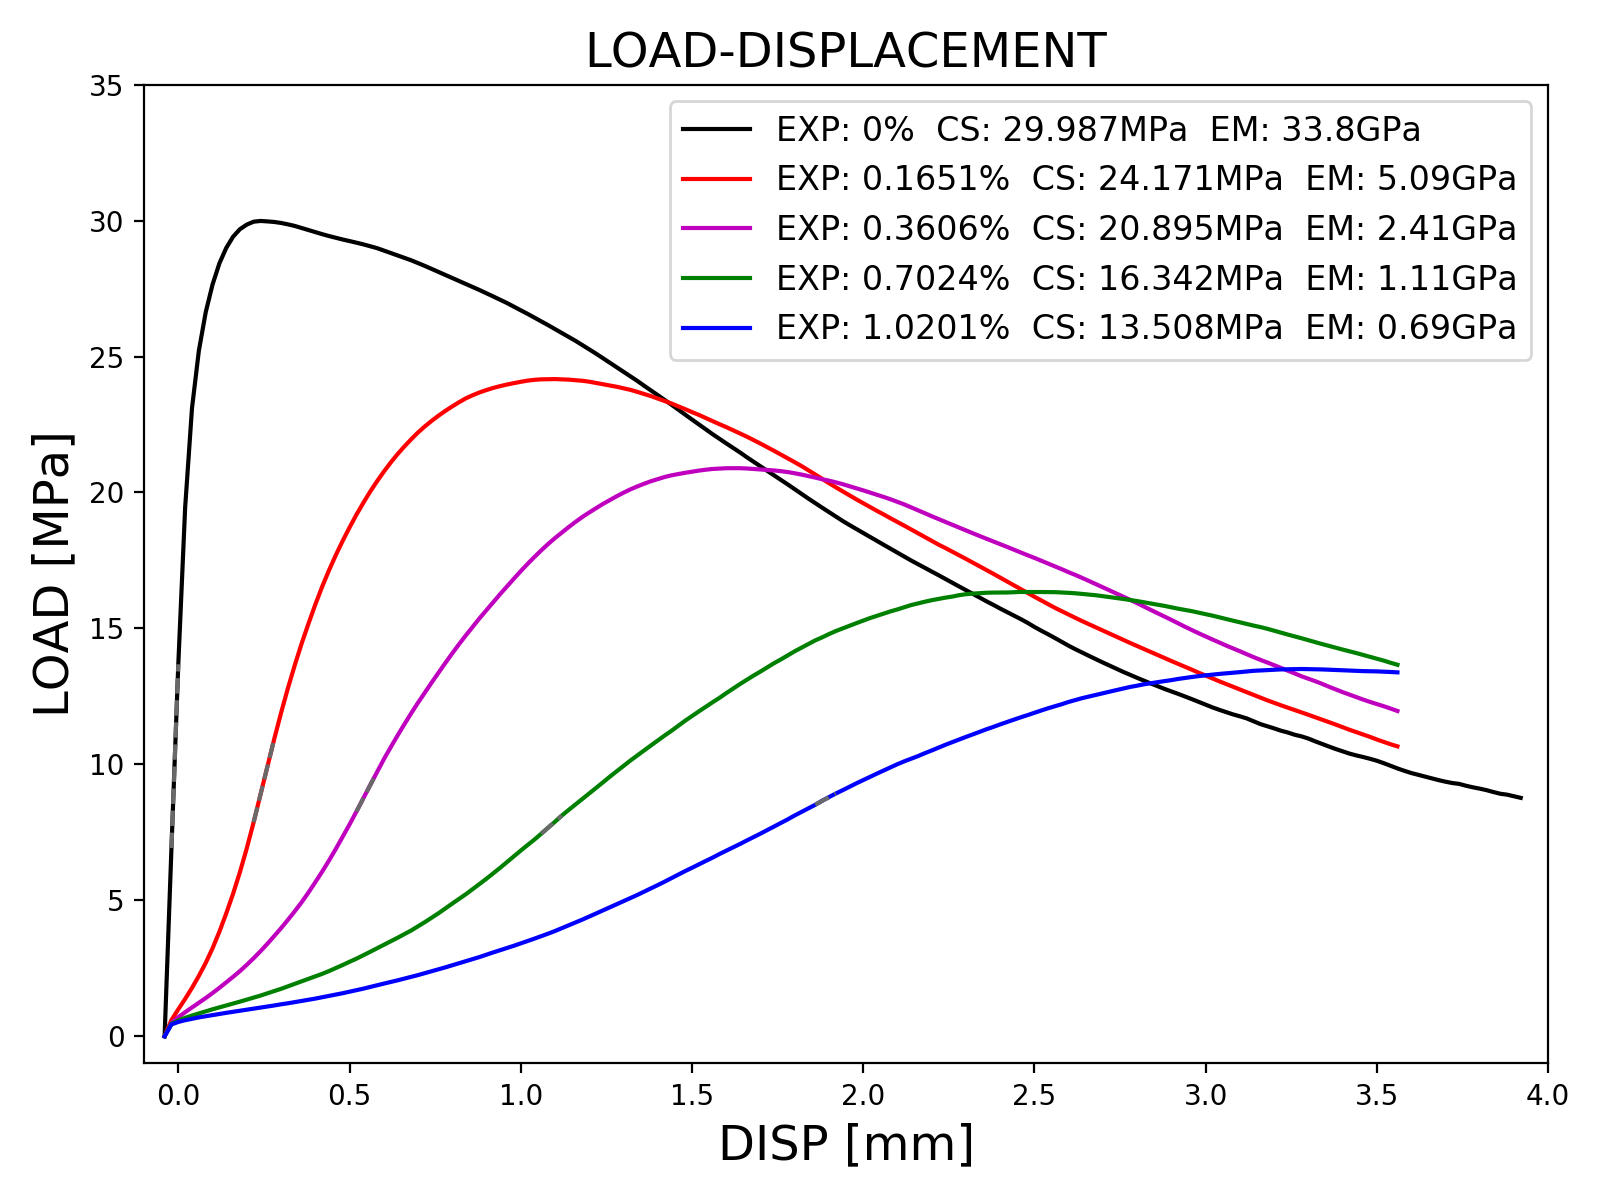
\includegraphics[width=.8\linewidth]{Files/exp_3D/ASR/S13A30P25FIX-LOAD-DISPLACEMENT.png}
  \caption{A30 P25 Fix Load-Displacement}
  \label{fig:A30P25FIX_LD}
\end{figure}

\clearpage

For ASR expanded model with 15\% coarse aggregate (of which 75\% are ASR reactive), shown in Figure \ref{fig:A15P75_model}, the Load-Displacement curve is shown in Figure \ref{fig:A15P75FIX_LD}.

%A15P75FIX

\begin{figure}[ht]
\centering
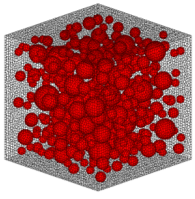
\includegraphics[width=.3\linewidth]{Files/Aggregate/A15.png}
  \caption{15\% Coarse Aggregate}
  \label{fig:A15P75_model}
\end{figure}

\begin{figure}[ht]
\centering
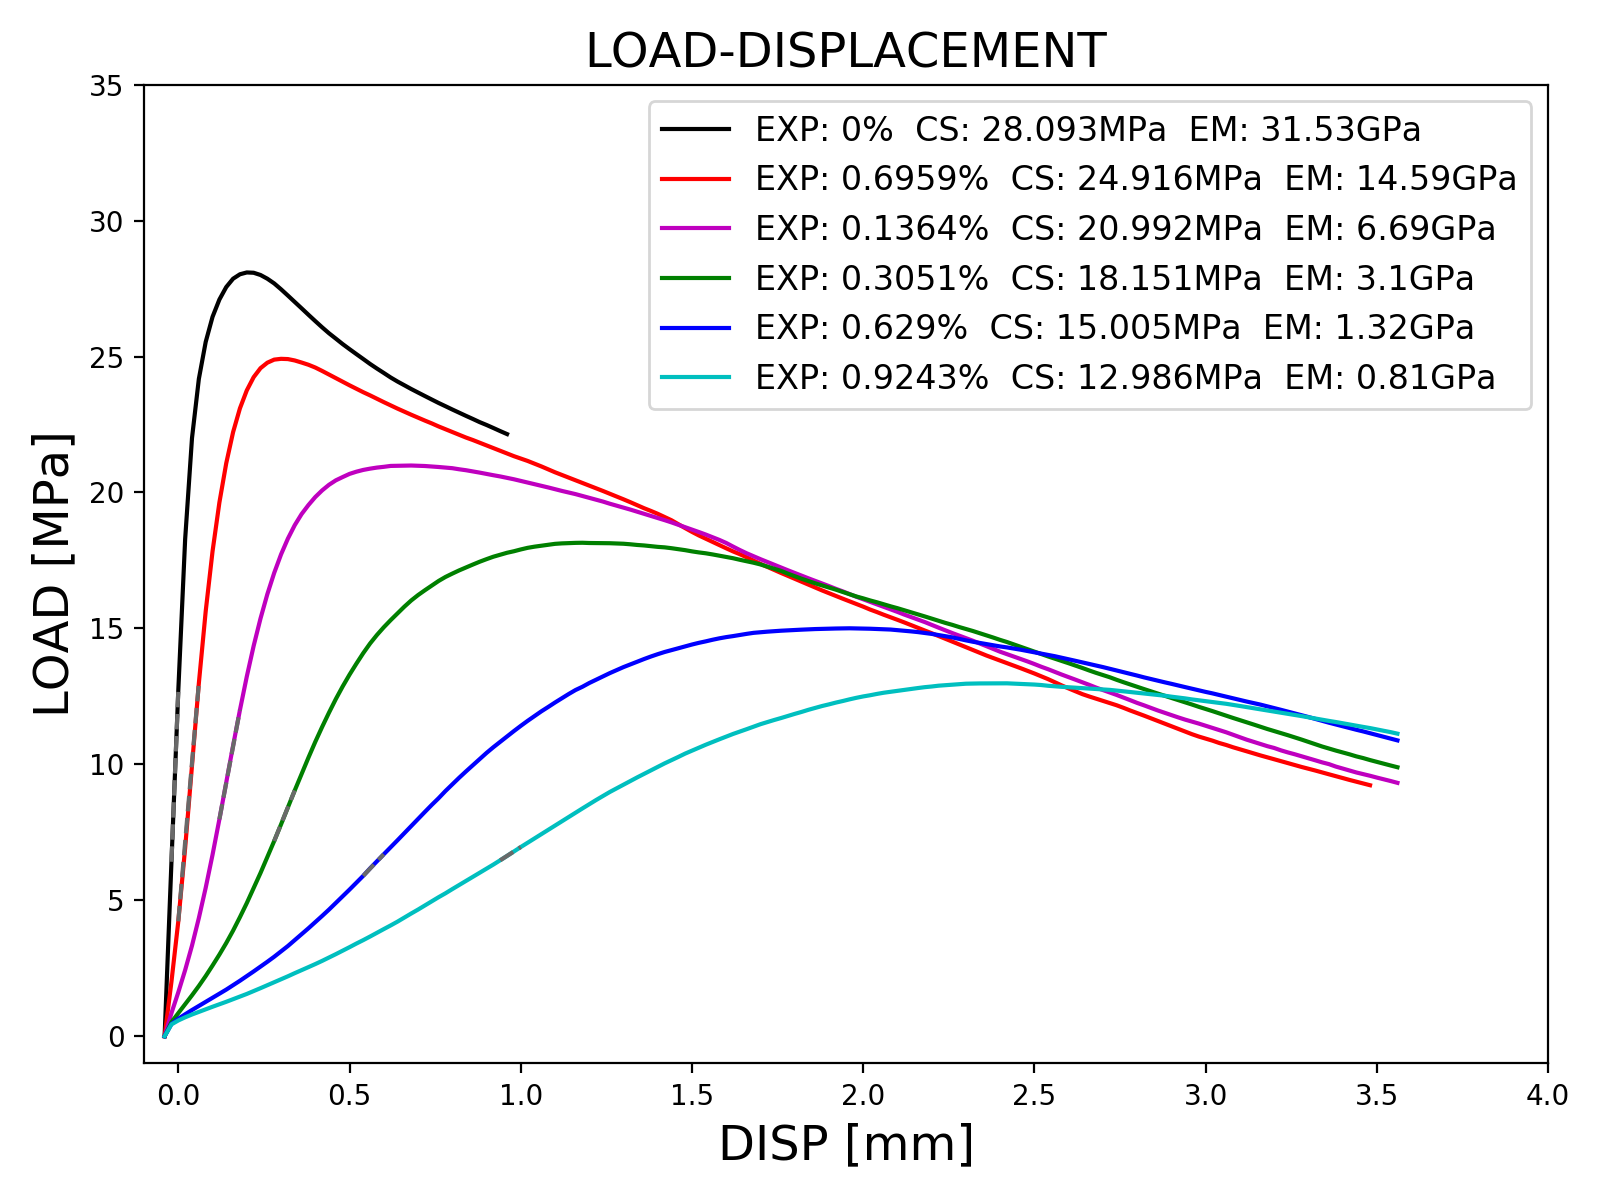
\includegraphics[width=.8\linewidth]{Files/exp_3D/ASR/S13A15P75FIX-LOAD-DISPLACEMENT.png}
  \caption{A15 P75 Fix Load-Displacement}
  \label{fig:A15P75FIX_LD}
\end{figure}

%TODO: PLOT WITH EXPERIMENTAL RESULTS
